\section{\PrintfSeveralArgumentsSectionName}

\IFRU{Попробуем теперь немного расширить пример \IT{\HelloWorldSectionName}~(\ref{sec:helloworld}),
написав в теле функции \main:}
{Now let's extend \IT{\HelloWorldSectionName}~(\ref{sec:helloworld}) example, replacing \printf in
the \main function body by this:}

\begin{lstlisting}
printf("a=%d; b=%d; c=%d", 1, 2, 3);
\end{lstlisting}

\section{x86: \RU{3 аргумента}\EN{3 arguments}}

\subsection{MSVC}

\RU{Компилируем при помощи MSVC 2010 Express, и в итоге получим:}
\EN{Let's compile it by MSVC 2010 Express and we got:}

\begin{lstlisting}
$SG3830	DB	'a=%d; b=%d; c=%d', 00H

...

	push	3
	push	2
	push	1
	push	OFFSET $SG3830
	call	_printf
	add	esp, 16					; 00000010H
\end{lstlisting}

\RU{Все почти то же, за исключением того, что теперь видно, что аргументы для \printf заталкиваются в стек в обратном порядке: самый первый аргумент заталкивается последним.}
\EN{Almost the same, but now we can see the \printf arguments are pushed onto the stack in reverse order. The first argument is pushed last.}

\RU{Кстати, вспомним что переменные типа \Tint в 32-битной системе, как известно, имеет ширину 32 бита, это 4 байта}
\EN{By the way, variables of \Tint type in 32-bit environment have 32-bit width, that is 4 bytes}.

\RU{Итак, у нас всего 4 аргумента. $4*4 = 16$ ~--- именно 16 байт занимают в стеке указатель на строку плюс еще 3 числа типа \Tint.}
\EN{So, we have here 4 arguments. $4*4 = 16$~---they occupy exactly 16 bytes in the stack: a 32-bit pointer to a string and 3 numbers of type \Tint.}

\index{x86!\Instructions!ADD}
\index{x86!\Registers!ESP}
\index{cdecl}
\RU{Когда при помощи инструкции \TT{``ADD ESP, X''} корректируется \glslink{stack pointer}{указатель стека} \ESP 
после вызова какой-либо функции, зачастую можно сделать вывод о том, сколько аргументов 
у вызываемой функции было, разделив X на 4.}
\EN{When the \gls{stack pointer} (\ESP register) is changed back by the \TT{``ADD ESP, X''}
instruction after a function 
call, often, the number of function arguments can be deduced here: just divide X by 4.}

\RU{Конечно, это относится только к cdecl-методу передачи аргументов через стек.}
\EN{Of course, this is specific to the \IT{cdecl} calling convention.}

\RU{См. также в соответствующем разделе о способах передачи аргументов через стек}
\EN{See also the section about calling conventions}~(\ref{sec:callingconventions}).

\RU{Иногда бывает так, что подряд идут несколько вызовов разных функций, 
но стек корректируется только один раз, после последнего вызова:}
\EN{It is also possible for the compiler to merge several \TT{``ADD ESP, X''} instructions into one, after the last call:}

\begin{lstlisting}
push a1
push a2
call ...
...
push a1
call ...
...
push a1
push a2
push a3
call ...
add esp, 24
\end{lstlisting}

\subsection{MSVC \AndENRU \olly}
\index{\olly}

\RU{Попробуем этот же пример в}\EN{Now let's try to load this example in} \olly.
\RU{Это один из наиболее популярных win32-отладчиков user-режима}\EN{It is one of the most 
popular user-land win32 debugger}.
\RU{Мы можем компилировать наш пример в}\EN{We can try to compile our example in} MSVC 2012 
\RU{с опцией}\EN{with} \TT{/MD} \RU{что означает, линковать с библиотекой}\EN{option, meaning, to link 
against} \TT{MSVCR*.DLL},
\RU{чтобы импортируемые ф-ции были хорошо видны в отладчике}\EN{so we will able to see imported 
functions clearly in the debugger}.

\RU{Затем загружаем исполняемый файл в}\EN{Then load executable in} \olly.
\RU{Самый первый брякпойнт в}\EN{The very first breakpoint is in} \TT{ntdll.dll}, \RU{нажмите}\EN{press} 
F9 (\RU{запустить}\EN{run}).
\RU{Второй брякпойнт в}\EN{The second breakpoint is in} \ac{CRT}-\RU{коде}\EN{code}.
\RU{Теперь мы должны найти ф-цию}\EN{Now we should find the} \main\EN{ function}.

\RU{Найдите этот код скроллируя окно кода до самого верха (MSVC располагает ф-цию \main в самом начале
секции кода)}\EN{Find this code by scrolling the code to the very top (MSVC allocates \main function at
the very beginning of the code section)}: 
\figref{fig:printf3_olly_1}.\\
\\
\RU{Кликните на инструкции}\EN{Click on the} \TT{PUSH EBP}\RU{, нажмите}\EN{ instruction, press} F2 
(\RU{установка брякпойнта}\EN{set breakpoint}) \RU{и нажмите}\EN{and press} F9 (\RU{запустить}\EN{run}).
\RU{Нам нужно произвести все эти манипуляции, чтобы пропустить \ac{CRT}-код, потому что нам он пока
не интересен}\EN{We need to do these manipulations in order to skip \ac{CRT}-code, because, we aren't really
interested in it, yet}.\\
\\
\RU{Нажмите}\EN{Press} F8 (\stepover) 6 \RU{раз, т.е., пропустить
6 инструкций}\EN{times, i.e., skip 6 instructions}: \figref{fig:printf3_olly_2}.\\
\\
\RU{Теперь}\EN{Now the} \ac{PC} \RU{указывает на инструкцию}\EN{points to the}
\TT{CALL printf}\EN{ instruction}.
\olly, \RU{как и другие отладчики, подсвечивает регистры со значениями, которые изменились}
\EN{like other debuggers, highlights value of registers which were changed}.
\RU{Так что, каждый раз, когда мы нажимаем}\EN{So each time you press F8}, \EIP 
\RU{изменяется и его значение подсвечивается красным}\EN{ changes and its value looks red}.
\ESP \RU{также меняется, потому что значения заталкиваются в стек}\EN{changes as well, 
because values are pushed into the stack}.\\
\\
\RU{Где находятся эти значения в стеке}\EN{Where are the values in the stack}?
\RU{Посмотрите на правое/нижнее окно в отладчике}\EN{Take a look at the right/bottom window of debugger}:

\begin{figure}[H]
\centering
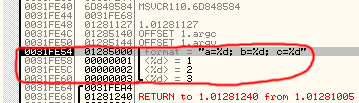
\includegraphics[scale=0.66]{patterns/03_printf/olly3_stack.png}
\caption{\olly: \RU{стек, после того как значения там сохранены}\EN{stack after values pushed}
(\RU{я сделал здесь округлую красную пометку в графическом редакторе}\EN{I made the round red mark 
here in a graphics editor})}
\end{figure}

\RU{Так что здесь видно 3 столбца: адрес в стеке, значение в стеке и еще дополнительный комментарий
от \olly}\EN{So we can see 3 columns there: address in the stack, 
value in the stack and some additional \olly comments}. 
\olly \RU{понимает}\EN{understands} \printf\RU{-строки}\EN{-like strings}, 
\RU{так что он показывает здесь и строку и 3 значения \IT{привязанных} к ней}\EN{so it reports the 
string here and 3 values \IT{attached} to it}.

\RU{Можно кликнуть правой кнопкой мыши на строке формата, кликнуть на ``Follow in dump''
и строка формата появится в окне слева внизу, где всегда виден какой-либо участок памяти}
\EN{It is possible to right-click on the format string, click on ``Follow in dump'',
and the format string will appear in the window at the left-bottom part, where some memory part
is always seen}.
\RU{Эти значения в памяти можно редактировать}\EN{These memory values can be edited}.
\RU{Можно изменить саму строку формата, и тогда результат работы нашего примера будет другой}
\EN{It is possible to change the format string, and then the result of our example will be different}.
\RU{В данном случае, пользы от этого немного, но для упражнения это полезно,
чтобы начать чувствовать как тут всё работает}\EN{It is probably not very useful now, but it's a very
good idea for doing it as an exercise, to get a feeling of how everything works here}.

\RU{Нажмите}\EN{Press} F8 (\stepover).

\RU{В консоли мы видим вывод}\EN{In the console we'll see the output}:

\begin{figure}[H]
\centering
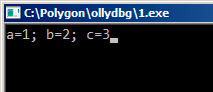
\includegraphics[scale=0.66]{patterns/03_printf/olly3_console.png}
\caption{\RU{Ф-ция }\printf \RU{исполнилась}\EN{function executed}}
\end{figure}

\RU{Посмотрим, как изменились регистры и состояние стека}\EN{Let's see how registers and stack state 
are changed}: \figref{fig:printf3_olly_3}.

\RU{Регистр }\EAX \RU{теперь содержит}\EN{register now contains} \TT{0xD} (13).
That's correct, since \printf returns the number of characters printed. The
\RU{Значение }\EIP \RU{изменилось: действительно, теперь здесь адрес инструкции после}
\EN{value is changed: indeed, now there is the address of the instruction after} \TT{CALL printf}.
\RU{Значения регистров }\ECX \AndENRU \EDX \RU{также изменились}\EN{values are changed as well}.
\RU{Очевидно, внутренности ф-ции \printf используют их для каких-то своих нужд}\EN{Apparently, 
\printf function's hidden machinery used them for its own needs}.

\RU{Очень важный момент в том что значение \ESP не изменилось. И аргменты-значения в стеке также!}
\EN{A very important fact is that neither the \ESP value, nor the stack state is changed!}
\RU{Мы ясно видим здесь и строку формата и соответствующие ей 3 значения, они все еще здесь.}
\EN{We clearly see that the format string and corresponding 3 values are still there.}
\RU{Действительно, по соглашению вызовов \IT{cdecl}, вызываемая ф-ция не возвращает \ESP назад.}
\EN{Indeed, that's the \IT{cdecl} calling convention: \gls{callee} doesn't return \ESP back to its previous value.}
\RU{Это должна делать вызывающая ф-ция}\EN{It's the \gls{caller}'s duty to do so}.

\RU{Нажмите}\EN{Press} F8 \RU{снова, чтобы исполнилась инструкция}\EN{again to execute} 
\TT{ADD ESP, 10}\EN{ instruction}: \figref{fig:printf3_olly_4}.

\ESP \RU{изменился, но значения все еще в стеке}\EN{is changed, but the values are still in the stack}!
\RU{Конечно, никому не нужно заполнять эти значения нулями или что-то в этом роде}\EN{Yes, 
of course; no one needs to fill these values by zero or something like that}.
\RU{Потому что всё что выше указателя стека}\EN{Because everything above stack pointer} (\ac{SP}) 
\RU{это}\EN{is} \IT{\RU{шум}\EN{noise}} \OrENRU \IT{\RU{мусор}\EN{garbage}}, \RU{это всё не имеет
особой ценности}\EN{and has no meaning at all}.
\RU{Было бы очень затратно по времени очищать ненужные элементы стека, к тому же, никому это и не 
нужно}\EN{It would be time consuming to clear unused stack entries anyways, and no one really needs to}.

\begin{figure}[H]
\centering
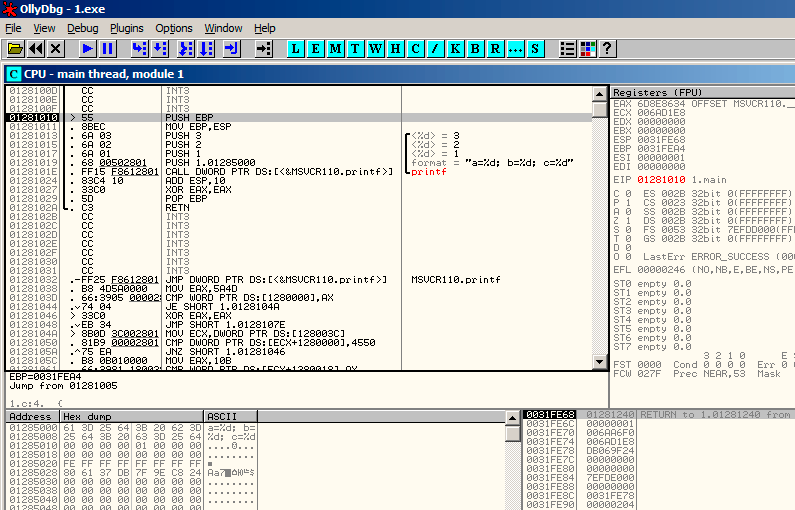
\includegraphics[scale=\FigScale]{patterns/03_printf/olly3_1.png}
\caption{\olly: \RU{самое начало ф-ции}\EN{the very start of the} \main\EN{ function}}
\label{fig:printf3_olly_1}
\end{figure}

\begin{figure}[H]
\centering
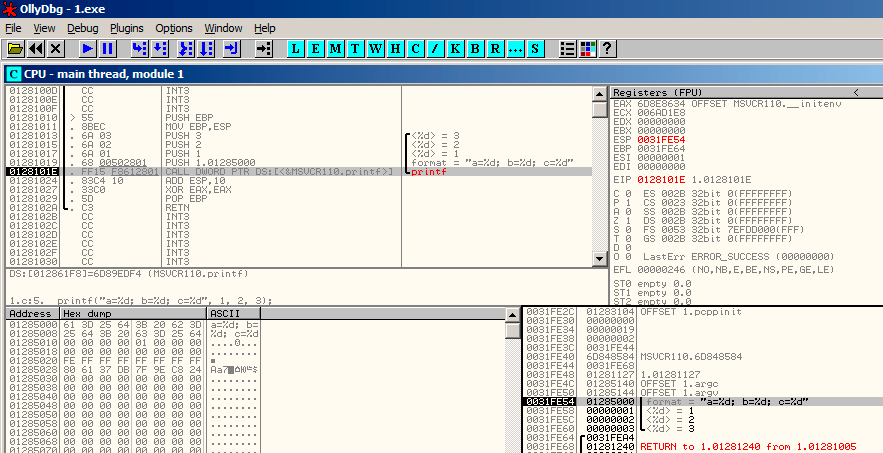
\includegraphics[scale=\FigScale]{patterns/03_printf/olly3_2.png}
\caption{\olly: \RU{перед исполнением}\EN{before} \printf\EN{ execution}}
\label{fig:printf3_olly_2}
\end{figure}

\begin{figure}[H]
\centering
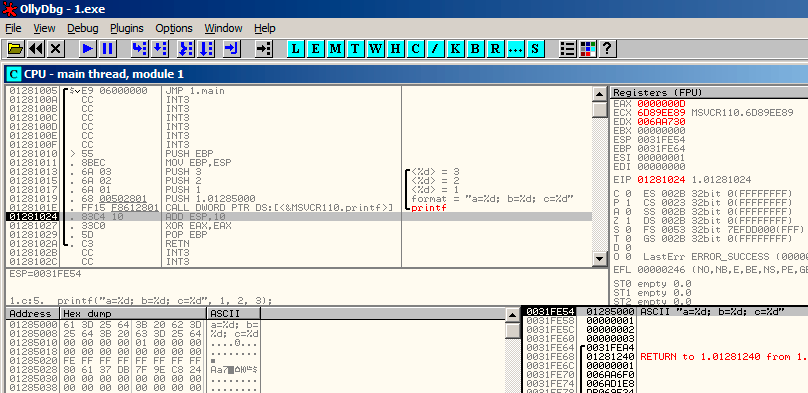
\includegraphics[scale=\FigScale]{patterns/03_printf/olly3_3.png}
\caption{\olly: \RU{после исполнения}\EN{after} \printf\EN{ execution}}
\label{fig:printf3_olly_3}
\end{figure}

\begin{figure}[H]
\centering
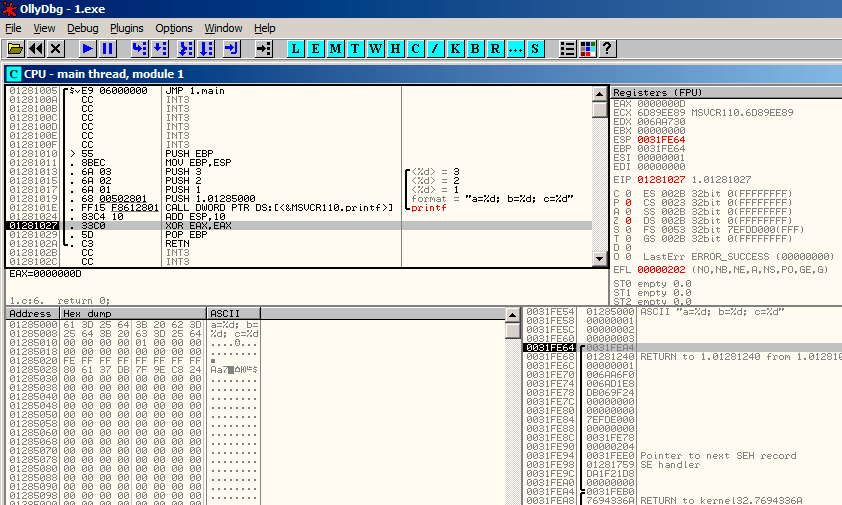
\includegraphics[scale=\FigScale]{patterns/03_printf/olly3_4.png}
\caption{\olly: \RU{после исполнения инструкции}\EN{after} \TT{ADD ESP, 10}\EN{ instruction execution}}
\label{fig:printf3_olly_4}
\end{figure}

\subsection{GCC}

\RU{Скомпилируем то же самое в Linux при помощи GCC 4.4.1 и посмотрим в \IDA что вышло:}
\EN{Now let's compile the same program in Linux using GCC 4.4.1 and take a look in \IDA what we got:}

\begin{lstlisting}
main            proc near

var_10          = dword ptr -10h
var_C           = dword ptr -0Ch
var_8           = dword ptr -8
var_4           = dword ptr -4

                push    ebp
                mov     ebp, esp
                and     esp, 0FFFFFFF0h
                sub     esp, 10h
                mov     eax, offset aADBDCD ; "a=%d; b=%d; c=%d"
                mov     [esp+10h+var_4], 3
                mov     [esp+10h+var_8], 2
                mov     [esp+10h+var_C], 1
                mov     [esp+10h+var_10], eax
                call    _printf
                mov     eax, 0
                leave
                retn
main            endp
\end{lstlisting}

\RU{Можно сказать, что этот короткий код, созданный GCC, отличается от кода MSVC только способом помещения 
значений в стек.
Здесь GCC снова работает со стеком напрямую без \PUSH/\POP.}
\EN{It can be said that the difference between code from MSVC and code from GCC is only in the method of placing arguments on the stack.
Here GCC is working directly with the stack without \PUSH/\POP.}

\subsection{GCC \AndENRU GDB}
\index{GDB}

\RU{Попробуем также этот пример и в \ac{GDB} в Linux}\EN{Let's try this example also in \ac{GDB} in Linux}.

\TT{-g} \RU{означает генерировать отладочную информацию в выходном исполняемом файле}\EN{mean produce 
debug information into executable file}.

\begin{lstlisting}
$ gcc 1.c -g -o 1
\end{lstlisting}

\begin{lstlisting}
$ gdb 1
GNU gdb (GDB) 7.6.1-ubuntu
Copyright (C) 2013 Free Software Foundation, Inc.
License GPLv3+: GNU GPL version 3 or later <http://gnu.org/licenses/gpl.html>
This is free software: you are free to change and redistribute it.
There is NO WARRANTY, to the extent permitted by law.  Type "show copying"
and "show warranty" for details.
This GDB was configured as "i686-linux-gnu".
For bug reporting instructions, please see:
<http://www.gnu.org/software/gdb/bugs/>...
Reading symbols from /home/dennis/polygon/1...done.
\end{lstlisting}

\begin{lstlisting}[caption=\RU{установим брякпойнт на}\EN{let's set breakpoint on} \printf]
(gdb) b printf
Breakpoint 1 at 0x80482f0
\end{lstlisting}

\RU{Запукаем}\EN{Run}.
\RU{Здесь у нас нет исходного кода ф-ции}\EN{There are no} \printf 
\RU{так что \ac{GDB} не может показать его исходный код, но могла бы}\EN{function source code here, 
so \ac{GDB} can't show its source, but may do so}.

\begin{lstlisting}
(gdb) run
Starting program: /home/dennis/polygon/1 

Breakpoint 1, __printf (format=0x80484f0 "a=%d; b=%d; c=%d") at printf.c:29
29	printf.c: No such file or directory.
\end{lstlisting}

\RU{Выдать 10 элементов стека. Левый столбец это адрес в стеке.}
\EN{Print 10 stack elements. The left column is an address in stack.}

\begin{lstlisting}
(gdb) x/10w $esp
0xbffff11c:	0x0804844a	0x080484f0	0x00000001	0x00000002
0xbffff12c:	0x00000003	0x08048460	0x00000000	0x00000000
0xbffff13c:	0xb7e29905	0x00000001
\end{lstlisting}

\RU{Самый первый элемент это}\EN{The very first element is the} \ac{RA} (\TT{0x0804844a}).
\RU{Мы можем удостовериться в этом, дизассемблируя память по этому адресу}\EN{We can make sure 
by disassembling the memory at this address}:

\begin{lstlisting}
(gdb) x/5i 0x0804844a
   0x804844a <main+45>:	mov    $0x0,%eax
   0x804844f <main+50>:	leave  
   0x8048450 <main+51>:	ret    
   0x8048451:	xchg   %ax,%ax
   0x8048453:	xchg   %ax,%ax
\end{lstlisting}

\RU{Две инструкции}\EN{Two} \TT{XCHG} 
\RU{это, вероятно, какой-то случайный мусор, который мы пока что можем игнорировать}
\EN{instructions, apparently, is some random garbage, which we can ignore so far}.

\RU{Второй элемент}\EN{The second element} (\TT{0x080484f0}) \RU{это адрес
строки формата}\EN{is an address of format string}:

\begin{lstlisting}
(gdb) x/s 0x080484f0
0x80484f0:	"a=%d; b=%d; c=%d"
\end{lstlisting}

\RU{Остальные 3 элемента}\EN{Other 3 elements} (1, 2, 3) \RU{это аргументы ф-ции}\EN{are} 
\printf\EN{ arguments}.
\RU{Остальные элементы это может быть и мусор в стеке, но могут быть и значения
от других ф-ций, их локальные переменные, итд}\EN{Other elements may be just ``garbage'' present in stack,
but also may be values from other functions, their local variables, etc}.
\RU{Пока что мы можем игнорировать их}\EN{We can ignore it for now}.

\RU{Исполняем}\EN{Execute} ``finish''. 
\RU{Это значит, исполнять до конца ф-ции}\EN{This mean, execute till function end}. 
\RU{Здесь это означает: исполнять до завершения}\EN{Here it means: execute till the finish of} \printf.

\begin{lstlisting}
(gdb) finish
Run till exit from #0  __printf (format=0x80484f0 "a=%d; b=%d; c=%d") at printf.c:29
main () at 1.c:6
6		return 0;
Value returned is $2 = 13
\end{lstlisting}

\ac{GDB} \RU{показывает, что вернула}\EN{shows what} \printf \RU{в}\EN{returned in} \EAX (13).
\RU{Это, так же как и в примере с \olly, количество напечатанных символов}
\EN{This is number of characters printed, just like in the example with \olly}.

\RU{А еще мы видим}\EN{We also see} ``return 0;'' \RU{и что это выражение находится в файле 
\TT{1.c} в строке 6}\EN{and the information that this expression is in the \TT{1.c} file at the line 6}.
\RU{Действительно, файл \TT{1.c} лежит в текущем директории и \ac{GDB} находит там эту строку}
\EN{Indeed, the \TT{1.c} file is located in the current directory, and \ac{GDB} finds the string there}.
\RU{Как \ac{GDB} знает, какая строка Си-кода сейчас исполняется}\EN{How does \ac{GDB} know which C-code line
is being executed now}?
\RU{Это связано с тем фактом, что компилятор, генерируя отладочную информацию,
также сохраняет информацию о 
соответствии строк в исходном коде и адресов инструкций}\EN{This is due to the fact that the compiler,
while generating debugging information, also saves a table of relations between source code line
numbers and instruction addresses}.
GDB \RU{это всё-таки отладчик уровня исходных текстов}\EN{is a source-level debugger, after all}.

\RU{Посмотрим регистры}\EN{Let's examine registers}.
13 \InENRU \EAX:

\begin{lstlisting}
(gdb) info registers
eax            0xd	13
ecx            0x0	0
edx            0x0	0
ebx            0xb7fc0000	-1208221696
esp            0xbffff120	0xbffff120
ebp            0xbffff138	0xbffff138
esi            0x0	0
edi            0x0	0
eip            0x804844a	0x804844a <main+45>
...
\end{lstlisting}

\RU{Попробуем дизассемблировать текущие инструкции}\EN{Let's disassemble the current instructions}.
\RU{Стрелка указывает на инструкцию, которая будет исполнена следующей}\EN{The arrow points to the 
instruction to be executed next}.

\begin{lstlisting}
(gdb) disas
Dump of assembler code for function main:
   0x0804841d <+0>:	push   %ebp
   0x0804841e <+1>:	mov    %esp,%ebp
   0x08048420 <+3>:	and    $0xfffffff0,%esp
   0x08048423 <+6>:	sub    $0x10,%esp
   0x08048426 <+9>:	movl   $0x3,0xc(%esp)
   0x0804842e <+17>:	movl   $0x2,0x8(%esp)
   0x08048436 <+25>:	movl   $0x1,0x4(%esp)
   0x0804843e <+33>:	movl   $0x80484f0,(%esp)
   0x08048445 <+40>:	call   0x80482f0 <printf@plt>
=> 0x0804844a <+45>:	mov    $0x0,%eax
   0x0804844f <+50>:	leave  
   0x08048450 <+51>:	ret    
End of assembler dump.
\end{lstlisting}

\ac{GDB} \RU{показывает дизассемблированный листинг в формате}\EN{shows disassembly in} AT\&T 
\RU{по умолчанию}\EN{syntax by default}.
\RU{Но можно также переключиться в формат Intel}\EN{It's possible to switch to Intel syntax}:

\begin{lstlisting}
(gdb) set disassembly-flavor intel
(gdb) disas
Dump of assembler code for function main:
   0x0804841d <+0>:	push   ebp
   0x0804841e <+1>:	mov    ebp,esp
   0x08048420 <+3>:	and    esp,0xfffffff0
   0x08048423 <+6>:	sub    esp,0x10
   0x08048426 <+9>:	mov    DWORD PTR [esp+0xc],0x3
   0x0804842e <+17>:	mov    DWORD PTR [esp+0x8],0x2
   0x08048436 <+25>:	mov    DWORD PTR [esp+0x4],0x1
   0x0804843e <+33>:	mov    DWORD PTR [esp],0x80484f0
   0x08048445 <+40>:	call   0x80482f0 <printf@plt>
=> 0x0804844a <+45>:	mov    eax,0x0
   0x0804844f <+50>:	leave  
   0x08048450 <+51>:	ret    
End of assembler dump.
\end{lstlisting}

\RU{Исполняем следующую инструкцию}\EN{Execute next instruction}.
\ac{GDB} \RU{покажет закрывающуюся скобку, означая, что это конец блока в ф-ции}\EN{shows ending bracket, 
meaning, this ends the block of the function}.

\begin{lstlisting}
(gdb) step
7	};
\end{lstlisting}

\RU{Посмотрим регистры после исполнения инструкции}\EN{Let's see the registers after the} 
\TT{MOV EAX, 0}\EN{ instruction execution}.
\EAX \RU{здесь уже действительно ноль}\EN{here is zero indeed}.

\begin{lstlisting}
(gdb) info registers
eax            0x0	0
ecx            0x0	0
edx            0x0	0
ebx            0xb7fc0000	-1208221696
esp            0xbffff120	0xbffff120
ebp            0xbffff138	0xbffff138
esi            0x0	0
edi            0x0	0
eip            0x804844f	0x804844f <main+50>
...
\end{lstlisting}

\section{ARM: \IFRU{3 аргумента}{3 arguments}}

\IFRU{В ARM традиционно принята такая схема передачи аргументов в функцию: 
4 первых аргумента через регистры \Reg{0}-\Reg{3}; а остальные ~--- через стек}
{Traditionally, ARM's scheme for passing arguments (calling convention) is as follows:
the first 4 arguments are passed in the \Reg{0}-\Reg{3} registers; the remaining arguments, via the stack}.
\IFRU{Это немного похоже на то, как аргументы передаются в}{This resembles the arguments passing scheme in} 
fastcall~(\ref{fastcall}) \OrENRU win64~(\ref{sec:callingconventions_win64}).

\subsection{\NonOptimizingKeil + \ARMMode}

\begin{lstlisting}[caption=\NonOptimizingKeil + \ARMMode]
.text:00000014             printf_main1
.text:00000014 10 40 2D E9   STMFD   SP!, {R4,LR}
.text:00000018 03 30 A0 E3   MOV     R3, #3
.text:0000001C 02 20 A0 E3   MOV     R2, #2
.text:00000020 01 10 A0 E3   MOV     R1, #1
.text:00000024 1D 0E 8F E2   ADR     R0, aADBDCD     ; "a=%d; b=%d; c=%d\n"
.text:00000028 0D 19 00 EB   BL      __2printf
.text:0000002C 10 80 BD E8   LDMFD   SP!, {R4,PC}
\end{lstlisting}

\IFRU{Итак, первые 4 аргумента передаются через регистры \Reg{0}-\Reg{3}, по порядку: 
указатель на формат-строку для \printf
в \Reg{0}, затем $1$ в \Reg{1}, $2$ в \Reg{2} и $3$ в \Reg{3}}
{So, the first 4 arguments are passed via the \Reg{0}-\Reg{3} registers in this order:
a pointer to the \printf format string in 
\Reg{0}, then $1$ in \Reg{1}, $2$ in \Reg{2} and $3$ in \Reg{3}}.

\IFRU{Пока что здесь нет ничего необычного}{There is nothing unusual so far}.

\subsection{\OptimizingKeil + \ARMMode}
\label{ARM_B_to_printf}

\begin{lstlisting}[caption=\OptimizingKeil + \ARMMode]
.text:00000014               EXPORT printf_main1
.text:00000014             printf_main1
.text:00000014 03 30 A0 E3   MOV     R3, #3
.text:00000018 02 20 A0 E3   MOV     R2, #2
.text:0000001C 01 10 A0 E3   MOV     R1, #1
.text:00000020 1E 0E 8F E2   ADR     R0, aADBDCD     ; "a=%d; b=%d; c=%d\n"
.text:00000024 CB 18 00 EA   B       __2printf
\end{lstlisting}

\index{ARM!\Registers!Link Register}
\index{ARM!\Instructions!B}
\index{Function epilogue}
\IFRU{Это соптимизированная версия (\Othree) для режима ARM, и здесь мы видим последнюю инструкцию: 
\TT{B} вместо привычной нам \TT{BL}}{This is optimized (\Othree) version for ARM mode and here we see \TT{B} as
the last instruction instead of the familiar \TT{BL}}.
\IFRU{Отличия между этой соптимизированной версией и предыдущей, скомпилированной без оптимизации, 
еще и в том, 
что здесь нет пролога и эпилога функции (инструкций, сохраняющих состояние регистров \TT{\Reg{0}} и \ac{LR})}
{Another difference between this optimized version and the previous one (compiled without optimization)
is also in the
fact that there is no function prologue and epilogue (instructions that save \TT{\Reg{0}} and \ac{LR} registers values)}.
\index{x86!\Instructions!JMP}
\IFRU{Инструкция \TT{B} просто переходит на другой адрес, без манипуляций с регистром \ac{LR}, то есть
это аналог \JMP в x86}
{The \TT{B} instruction just jumps to another address, without any manipulation of the \ac{LR} register,
that is, it is analogous to \JMP in x86}.
\IFRU{Почему это работает нормально? Потому что этот код эквивалентен предыдущему.}
{Why does it work? Because this code is, in fact, effectively equivalent to the previous.}
\IFRU{Основных причин две: 1) стек не модифицируется, как и \glslink{stack pointer}{указатель стека} \ac{SP}; 2) вызов функции \printf последний, 
после него ничего не происходит}{There are two main reasons: 1) neither the stack nor \ac{SP}, the \gls{stack pointer}, is modified;
2) the call to \printf is the last instruction, so there is nothing going on after it}.
\IFRU{Функция \printf, отработав, просто вернет управление по адресу, записанному в \ac{LR}}{After finishing, the \printf
function will just return control to the address stored in \ac{LR}}.
\IFRU{Но в \ac{LR} находится адрес места, откуда была вызвана наша функция}
{But the address of the point from where our function
was called is now in \ac{LR}}!
\IFRU{А следовательно, управление из \printf вернется сразу туда}
{Consequently, control from \printf will be returned to that point}.
\IFRU{Следовательно, нет нужды сохранять \ac{LR}, потому что нет нужны модифицировать \ac{LR}}
{As a consequence, we do not need to save \ac{LR} since we do not need to modify \ac{LR}}.
\IFRU{А нет нужды модифицировать \ac{LR}, потому что нет иных вызовов функций, кроме \printf, к тому же, после этого вызова не нужно ничего здесь больше делать}
{We do not need to modify \ac{LR} since there are no other function calls except \printf. Furthermore,
after this call we do not to do anything}!
\IFRU{Поэтому такая оптимизация возможна}
{That's why this optimization is possible}.

\IFRU{Еще один похожий пример описан в секции}{Another similar example was described in} 
``\SwitchCaseDefaultSectionName'' 
\IFRU{, здесь}{section, here}~(\ref{jump_to_last_printf}).

\subsection{\OptimizingKeil + \ThumbMode}

\begin{lstlisting}[caption=\OptimizingKeil + \ThumbMode]
.text:0000000C             printf_main1
.text:0000000C 10 B5         PUSH    {R4,LR}
.text:0000000E 03 23         MOVS    R3, #3
.text:00000010 02 22         MOVS    R2, #2
.text:00000012 01 21         MOVS    R1, #1
.text:00000014 A4 A0         ADR     R0, aADBDCD     ; "a=%d; b=%d; c=%d\n"
.text:00000016 06 F0 EB F8   BL      __2printf
.text:0000001A 10 BD         POP     {R4,PC}
\end{lstlisting}

\IFRU{Здесь нет особых отличий от неоптимизированного варианта для режима ARM}
{There is no significant difference from the non-optimized code for ARM mode}.



\section{ARM: \RU{8 аргументов}\EN{8 arguments}}

\RU{Снова воспользуемся примером с 9-ю аргументами из предыдущей секции}\EN{Let's use again the example
with 9 arguments from the previous section}: \ref{example_printf8_x64}.

\begin{lstlisting}
void printf_main2()
{
    printf("a=%d; b=%d; c=%d; d=%d; e=%d; f=%d; g=%d; h=%d\n", 
        1, 2, 3, 4, 5, 6, 7, 8);
};
\end{lstlisting}

\subsection{\OptimizingKeil: \ARMMode}

\begin{lstlisting}
.text:00000028             printf_main2
.text:00000028
.text:00000028             var_18 = -0x18
.text:00000028             var_14 = -0x14
.text:00000028             var_4  = -4
.text:00000028
.text:00000028 04 E0 2D E5  STR    LR, [SP,#var_4]!
.text:0000002C 14 D0 4D E2  SUB    SP, SP, #0x14
.text:00000030 08 30 A0 E3  MOV    R3, #8
.text:00000034 07 20 A0 E3  MOV    R2, #7
.text:00000038 06 10 A0 E3  MOV    R1, #6
.text:0000003C 05 00 A0 E3  MOV    R0, #5
.text:00000040 04 C0 8D E2  ADD    R12, SP, #0x18+var_14
.text:00000044 0F 00 8C E8  STMIA  R12, {R0-R3}
.text:00000048 04 00 A0 E3  MOV    R0, #4
.text:0000004C 00 00 8D E5  STR    R0, [SP,#0x18+var_18]
.text:00000050 03 30 A0 E3  MOV    R3, #3
.text:00000054 02 20 A0 E3  MOV    R2, #2
.text:00000058 01 10 A0 E3  MOV    R1, #1
.text:0000005C 6E 0F 8F E2  ADR    R0, aADBDCDDDEDFDGD ; "a=%d; b=%d; c=%d; d=%d; e=%d; f=%d; g=%"...
.text:00000060 BC 18 00 EB  BL     __2printf
.text:00000064 14 D0 8D E2  ADD    SP, SP, #0x14
.text:00000068 04 F0 9D E4  LDR    PC, [SP+4+var_4],#4
\end{lstlisting}

\RU{Этот код можно условно разделить на несколько частей}\EN{This code can be divided into several parts}:

\begin{itemize}
\index{Function prologue}
\item \RU{Пролог функции}\EN{Function prologue}:

\index{ARM!\Instructions!STR}
\RU{Самая первая инструкция}\EN{The very first} \TT{``STR LR, [SP,\#var\_4]!''} 
\RU{сохраняет в стеке \ac{LR}, ведь нам придется использовать этот регистр для вызова \printf}
\EN{instruction saves \ac{LR} on the stack, because we will use this register for the \printf call}.

\index{ARM!\Instructions!SUB}
\RU{Вторая инструкция}\EN{The second} \TT{``SUB SP, SP, \#0x14''}
\RU{уменьшает \glslink{stack pointer}{указатель стека} \ac{SP}, но, на самом деле, эта процедура нужна для выделения в локальном стеке места размером \TT{0x14} ($20$) байт}
\EN{instruction decreases
\ac{SP}, the \gls{stack pointer}, in order to 
allocate \TT{0x14} ($20$) bytes on the stack}.
\RU{Действительно, нам нужно передать 5 32-битных значений через стек в \printf, каждое значение занимает 4 байта, а $5*4=20$ ~--- как раз}
\EN{Indeed, we need to pass 5 32-bit values via the stack to the \printf function, and each one occupies 4 bytes, that is $5*4=20$~---exactly}.
\RU{Остальные 4 32-битных значения будут переданы через регистры}\EN{The other 4 32-bit values will be passed in
registers}.

\item \RU{Передача 5, 6, 7 и 8 через стек}\EN{Passing 5, 6, 7 and 8 via stack}:

\RU{Затем значения 5, 6, 7 и 8 записываются в регистры \Reg{0}, \Reg{1}, \Reg{2} и \Reg{3} соответственно}
\EN{Then, the values 5, 6, 7 and 8
are written to the \Reg{0}, \Reg{1}, \Reg{2} and \Reg{3} registers respectively}.
\RU{Затем инструкция}\EN{Then, the} \TT{``ADD R12, SP, \#0x18+var\_14''} 
\RU{записывает в регистр \TT{R12} адрес места в стеке, куда будут помещены эти 4 значения}
\EN{instruction writes an address of the point in the stack, where these 4 variables will be written, into the \TT{R12} register}.
\index{IDA!var\_?}
\IT{var\_14} \RU{~--- это макрос ассемблера}\EN{is an assembly macro}, \RU{равный}\EN{equal to} $-0x14$, 
\RU{такие макросы создает \IDA, чтобы удобнее было показывать, как код обращается к стеку}
\EN{such macros are created by \IDA to succinctly denote code accessing the stack}.
\RU{Макросы \IT{var\_?}, создаваемые \IDA, отражают локальные переменные в стеке}\EN{\IT{var\_?} macros created
by \IDA reflecting local variables in the stack}.
\RU{Так что в \TT{R12} будет записано $SP+4$}\EN{So, $SP+4$ will be written into the \TT{R12} register}.
\index{ARM!\Instructions!STMIA}
\RU{Следующая инструкция}\EN{The next} \TT{``STMIA R12, {R0-R3}''} 
\RU{записывает содержимое регистров \Reg{0}-\Reg{3} по адресу в памяти, на который указывает \TT{R12}}
\EN{instruction
writes \Reg{0}-\Reg{3} registers contents at the point in memory to which \TT{R12} pointing}.
\RU{Инструкция }\TT{STMIA} \RU{означает}\EN{instruction meaning} \IT{Store Multiple Increment After}. 
\IT{Increment After} \RU{означает, что \TT{R12} будет увеличиваться на 4 после записи каждого значения регистра}
\EN{means that \TT{R12} will be increased by $4$ after each register value is written}.

\item \RU{Передача $4$ через стек}\EN{Passing $4$ via stack}:
\RU{$4$ записывается в \Reg{0}, затем это значение при помощи инструкции}\EN{$4$ is stored in \Reg{0} and then,
this value, with the help of} \TT{``STR R0, [SP,\#0x18+var\_18]''} \RU{попадает в стек}\EN{instruction, is saved
on the stack}.
\IT{var\_18} \RU{равен}\EN{is} $-0x18$, \RU{смещение будет $0$}\EN{offset will be $0$}, 
\RU{так что, значение из регистра \Reg{0} ($4$) запишется туда, куда указывает \ac{SP}}
\EN{so, the value from the \Reg{0} register ($4$) will be written to the point where \ac{SP} is pointing to}.

\item \RU{Передача 1, 2 и 3 через регистры}\EN{Passing 1, 2 and 3 via registers}:

\RU{Значения для первых трех чисел (a, b, c) (1, 2, 3 соответственно) передаются в регистрах 
\Reg{1}, \Reg{2} и \Reg{3} перед самим вызовом \printf}
\EN{Values of the first 3 numbers (a, b, c) (1, 2, 3 respectively) are passed in the 
\Reg{1}, \Reg{2} and \Reg{3}
registers right before the \printf call}, \RU{а остальные 5 значений передаются через стек, и вот как}\EN{and the other
5 values are passed via the stack}:

\item \RU{Вызов \printf}\EN{\printf call}:

\index{Function epilogue}
\item \RU{Эпилог функции}\EN{Function epilogue}:

\RU{Инструкция}\EN{The} \TT{``ADD SP, SP, \#0x14''} \RU{возвращает \ac{SP} на прежнее место, 
аннулируя таким образом всё, что было записано в стеке}
\EN{instruction returns the \ac{SP} pointer back to its former point,
thus cleaning the stack}.
\RU{Конечно, то что было записано в стек, там пока и останется, но всё это будет многократно 
перезаписано во время исполнения последующих функций}
\EN{Of course, what was written on the stack will stay there, but it all will be
rewritten during the execution of subsequent functions}.

\index{ARM!\Instructions!LDR}
\RU{Инструкция}\EN{The} \TT{``LDR PC, [SP+4+var\_4],\#4''} \RU{загружает в \ac{PC} сохраненное значение \ac{LR} из стека,
обеспечивая таким образом выход из функции}
\EN{instruction loads the saved \ac{LR} value from the stack into the \ac{PC} register, thus causing
the function to exit}.

\end{itemize}

\subsection{\OptimizingKeil: \ThumbMode}

\begin{lstlisting}
.text:0000001C             printf_main2
.text:0000001C
.text:0000001C             var_18 = -0x18
.text:0000001C             var_14 = -0x14
.text:0000001C             var_8  = -8
.text:0000001C
.text:0000001C 00 B5        PUSH    {LR}
.text:0000001E 08 23        MOVS    R3, #8
.text:00000020 85 B0        SUB     SP, SP, #0x14
.text:00000022 04 93        STR     R3, [SP,#0x18+var_8]
.text:00000024 07 22        MOVS    R2, #7
.text:00000026 06 21        MOVS    R1, #6
.text:00000028 05 20        MOVS    R0, #5
.text:0000002A 01 AB        ADD     R3, SP, #0x18+var_14
.text:0000002C 07 C3        STMIA   R3!, {R0-R2}
.text:0000002E 04 20        MOVS    R0, #4
.text:00000030 00 90        STR     R0, [SP,#0x18+var_18]
.text:00000032 03 23        MOVS    R3, #3
.text:00000034 02 22        MOVS    R2, #2
.text:00000036 01 21        MOVS    R1, #1
.text:00000038 A0 A0        ADR     R0, aADBDCDDDEDFDGD ; "a=%d; b=%d; c=%d; d=%d; e=%d; f=%d; g=%"...
.text:0000003A 06 F0 D9 F8  BL      __2printf
.text:0000003E
.text:0000003E             loc_3E   ; CODE XREF: example13_f+16
.text:0000003E 05 B0        ADD     SP, SP, #0x14
.text:00000040 00 BD        POP     {PC}
\end{lstlisting}

\RU{Это почти то же самое, что и в предыдущем примере, только код для thumb и значения помещаются в 
стек немного иначе: в начале $8$ за первый раз, затем $5$, $6$, $7$ за второй раз и $4$ за третий раз}\EN{Almost 
same as
in previous example, however, this is thumb code and values are packed into stack differently: 
$8$ for the first time, then $5$, $6$, $7$ for the second and $4$ for the third}.

\subsection{\OptimizingXcode: \ARMMode}

\begin{lstlisting}
__text:0000290C             _printf_main2
__text:0000290C
__text:0000290C             var_1C = -0x1C
__text:0000290C             var_C  = -0xC
__text:0000290C
__text:0000290C 80 40 2D E9   STMFD  SP!, {R7,LR}
__text:00002910 0D 70 A0 E1   MOV    R7, SP
__text:00002914 14 D0 4D E2   SUB    SP, SP, #0x14
__text:00002918 70 05 01 E3   MOV    R0, #0x1570
__text:0000291C 07 C0 A0 E3   MOV    R12, #7
__text:00002920 00 00 40 E3   MOVT   R0, #0
__text:00002924 04 20 A0 E3   MOV    R2, #4
__text:00002928 00 00 8F E0   ADD    R0, PC, R0
__text:0000292C 06 30 A0 E3   MOV    R3, #6
__text:00002930 05 10 A0 E3   MOV    R1, #5
__text:00002934 00 20 8D E5   STR    R2, [SP,#0x1C+var_1C]
__text:00002938 0A 10 8D E9   STMFA  SP, {R1,R3,R12}
__text:0000293C 08 90 A0 E3   MOV    R9, #8
__text:00002940 01 10 A0 E3   MOV    R1, #1
__text:00002944 02 20 A0 E3   MOV    R2, #2
__text:00002948 03 30 A0 E3   MOV    R3, #3
__text:0000294C 10 90 8D E5   STR    R9, [SP,#0x1C+var_C]
__text:00002950 A4 05 00 EB   BL     _printf
__text:00002954 07 D0 A0 E1   MOV    SP, R7
__text:00002958 80 80 BD E8   LDMFD  SP!, {R7,PC}
\end{lstlisting}

\index{ARM!\Instructions!STMFA}
\index{ARM!\Instructions!STMIB}
\RU{Почти то же самое, что мы уже видели, за исключением того, что}
\EN{Almost the same what we already figured out, with the
exception of} \TT{STMFA} (Store Multiple Full Ascending) 
\RU{~--- это синоним инструкции}\EN{instruction, it is synonym to} 
\TT{STMIB} (Store Multiple Increment Before) \EN{instruction}. 
\RU{Эта инструкция увеличивает \ac{SP} и только затем записывает в память значение очередного регистра, 
но не наоборот}\EN{This
instruction increasing value in the \ac{SP} register and only then writing next register value into memory, but not vice versa}.

\RU{Второе, что бросается в глаза, это то, что инструкции как будто бы расположены случайно}\EN{Another thing
we easily spot is the instructions are ostensibly located randomly}.
\RU{Например, значение в регистре \Reg{0} подготавливается в трех местах, по адресам \TT{0x2918}, \TT{0x2920} 
и \TT{0x2928}, 
когда это можно было бы сделать в одном месте}\EN{For instance, value in the \Reg{0} register is prepared in three
places, at addresses \TT{0x2918}, \TT{0x2920} and \TT{0x2928}, when it would be possible to do it in one single point}.
\RU{Однако, у оптимизирующего компилятора могут быть свои доводы о том, как лучше составлять инструкции 
друг с другом для лучшей эффективности исполнения}
\EN{However, optimizing compiler has its own reasons about how
to place instructions better}.
\RU{Процессор обычно пытается исполнять одновременно идущие друг за другом инструкции}
\EN{Usually, processor attempts to simultaneously execute instructions located side-by-side}.
\RU{К примеру, инструкции}\EN{For example, instructions like} \TT{``MOVT R0, \#0''} \AndENRU 
\TT{``ADD R0, PC, R0''} \RU{не могут быть исполнены одновременно, потому что обе инструкции модифицируют 
регистр \Reg{0}}\EN{cannot be executed simultaneously since they both modifying the \Reg{0} register}. 
\RU{А вот инструкции}\EN{On the other hand,} \TT{``MOVT R0, \#0''} \AndENRU \TT{``MOV R2, \#4''} 
\RU{легко можно исполнить одновременно, 
потому что эффекты от их исполнения никак не конфликтуют друг с другом}\EN{instructions can be executed
simultaneously since effects of their execution are not conflicting with each other}.
\RU{Вероятно, компилятор старается генерировать код именно таким образом там, где это возможно}
\EN{Presumably, compiler tries to generate code in such a way, where it is possible, of course}.
 
\subsection{\OptimizingXcode: \ThumbTwoMode}

\begin{lstlisting}
__text:00002BA0               _printf_main2
__text:00002BA0
__text:00002BA0               var_1C = -0x1C
__text:00002BA0               var_18 = -0x18
__text:00002BA0               var_C  = -0xC
__text:00002BA0
__text:00002BA0 80 B5          PUSH     {R7,LR}
__text:00002BA2 6F 46          MOV      R7, SP
__text:00002BA4 85 B0          SUB      SP, SP, #0x14
__text:00002BA6 41 F2 D8 20    MOVW     R0, #0x12D8
__text:00002BAA 4F F0 07 0C    MOV.W    R12, #7
__text:00002BAE C0 F2 00 00    MOVT.W   R0, #0
__text:00002BB2 04 22          MOVS     R2, #4
__text:00002BB4 78 44          ADD      R0, PC  ; char *
__text:00002BB6 06 23          MOVS     R3, #6
__text:00002BB8 05 21          MOVS     R1, #5
__text:00002BBA 0D F1 04 0E    ADD.W    LR, SP, #0x1C+var_18
__text:00002BBE 00 92          STR      R2, [SP,#0x1C+var_1C]
__text:00002BC0 4F F0 08 09    MOV.W    R9, #8
__text:00002BC4 8E E8 0A 10    STMIA.W  LR, {R1,R3,R12}
__text:00002BC8 01 21          MOVS     R1, #1
__text:00002BCA 02 22          MOVS     R2, #2
__text:00002BCC 03 23          MOVS     R3, #3
__text:00002BCE CD F8 10 90    STR.W    R9, [SP,#0x1C+var_C]
__text:00002BD2 01 F0 0A EA    BLX      _printf
__text:00002BD6 05 B0          ADD      SP, SP, #0x14
__text:00002BD8 80 BD          POP      {R7,PC}
\end{lstlisting}

\RU{Почти то же самое, что и в предыдущем примере,
лишь за тем исключением, что здесь используются thumb-инструкции}
\EN{Almost the same as in previous example,
with the exception the thumb-instructions are used here instead}.



\subsection{\IFRU{Кстати}{By the way}}

\IFRU{Кстати, разница между способом передачи параметров принятая в x86 и ARM, неплохо иллюстрирует тот важный момент, что процессору, в общем, все равно как будут 
передаваться параметры функций. Можно создать гипотетический компилятор, который будет передавать их при 
помощи указателя на структуру с параметрами, не пользуясь стеком вообще.}
{By the way, this difference between passing arguments in x86 and ARM is a good illustration the CPU is not aware of how arguments is passed to functions. 
It is also possible to create hypothetical compiler which is able to pass arguments 
via a special structure not using stack at all.}

